\chapter {Analysis and Interpretation} 



All of the graphs are interpreted from raw data tables shown in the Experiment section of the coursework. Straight line graphs gradients are worked out from the straight line, and curved lines gradients are worked out by a red line extending from $t = 0$. The calculations are then shown below each graph. The graphs plotted take into account the fact that when the bung is pushed into the conical flask the volume of the system decreases which therefore increases the pressure and falsely reads on the gas syringe that hydrogen gas has been produced. Therefore the $Time = 0$ value for each data series has been taken away from every value, thus causing each series to pass through the origin.

\section{Zinc and Sulfuric Acid Without a Catalyst} 

Below are the graphs that I have used to work out the rate of the reaction for the experiment series that did not involve a catalyst. All graphs have taken a mean average of the three repeats in order to plot the data points. As discussed in my 'Chosen Method' section on page \pageref{Chosen Method} I am using the equation $Gradient = \frac{Change in Y}{Change in X}$ and as the gradient is equal to the rate of reaction, I will be able to use the graphs below in order to generate a rate vs concentration graph which will determine the order of the reaction. I will calculate all rates to 3 decimal places.

\begin{figure}[H]
    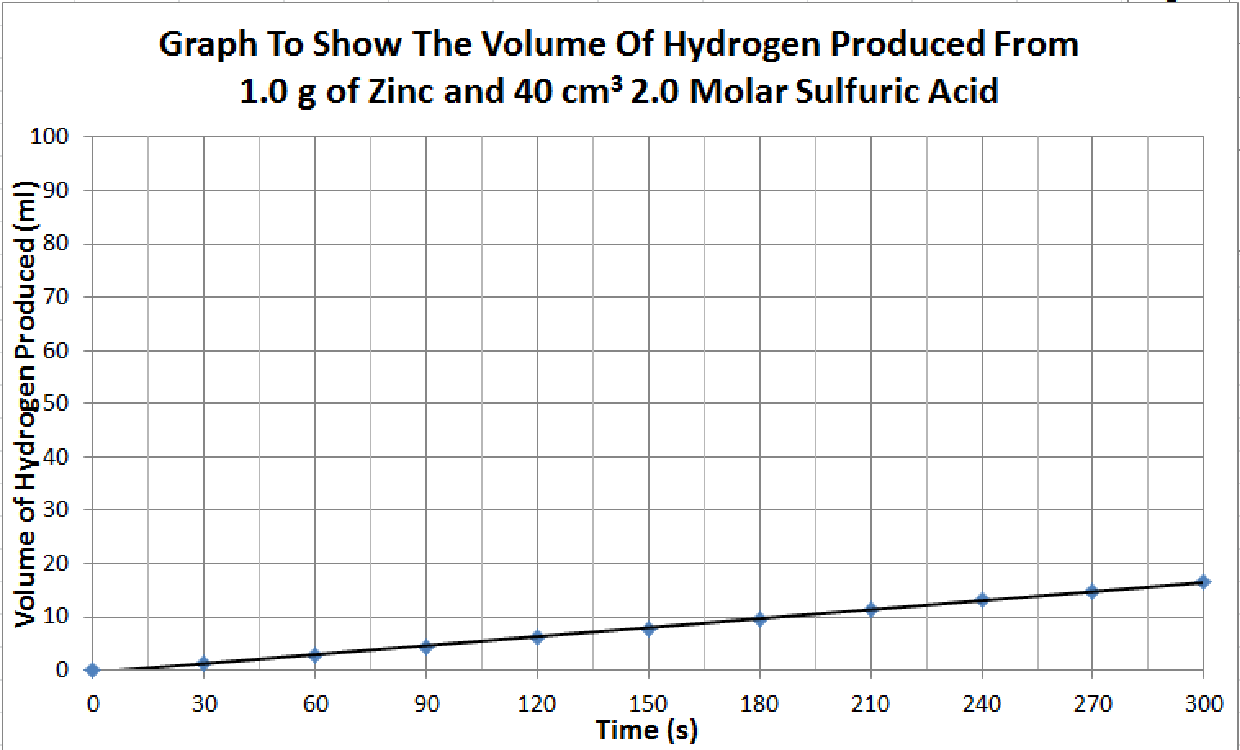
\includegraphics[width=\textwidth]{./Analysis/Images/1NonCatalyst/2Molar.pdf}
    \caption{2.0 Molar Sulfuric Acid and 1.0 g of Zinc Average Graph} \label{fig:2MolarSAGradient}
\end{figure}

$Gradient = \frac{16.67}{300}$

Therefore:

$Rate = 0.056 \; ml \; s^{-1}$

This graphs shape is similar to the majority of the graphs that I have produced. This steady, straight line can be explained by the fact that there is still the maximum amount of reactants available to react over the period of time that my experiment was taken. Eventually, if the graph continued, you would see the graph start to curve off due to less reactant molecules being available to react and therefore less likely for molecules to collide per unit time.

\begin{figure}[H]
    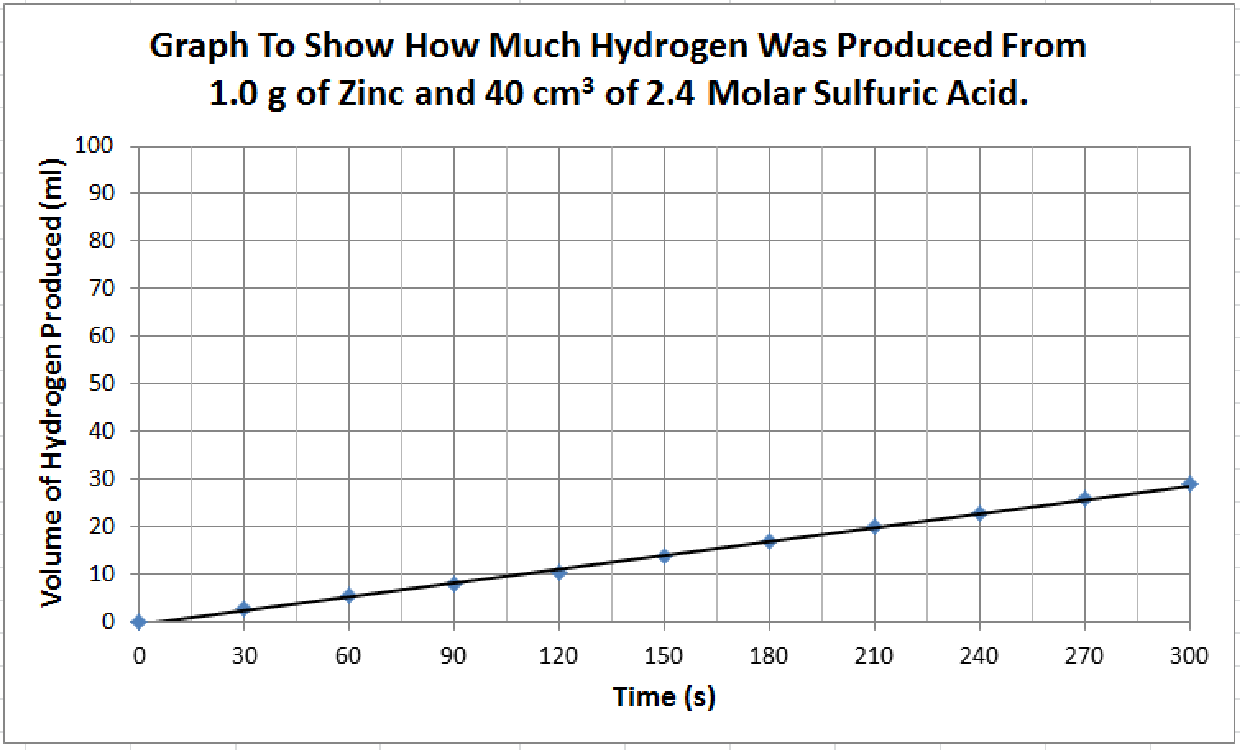
\includegraphics[width=\textwidth]{./Analysis/Images/1NonCatalyst/24Molar.pdf}
    \caption{2.4 Molar Sulfuric Acid and 1.0 g of Zinc Average Graph} \label{fig:24MolarSAGradient}
\end{figure}

$Gradient = \frac{28.83}{300}$

Therefore:

$Rate = 0.096 \; ml \; s^{-1}$

\begin{figure}[H]
    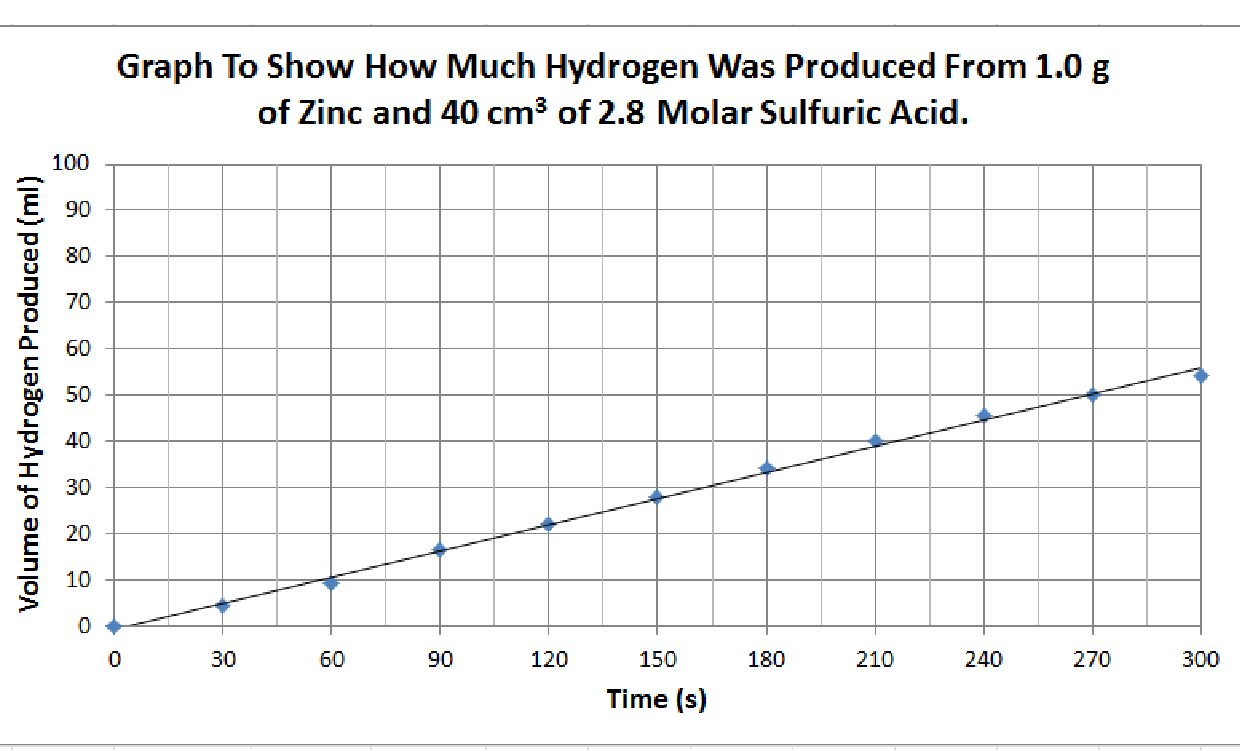
\includegraphics[width=\textwidth]{./Analysis/Images/1NonCatalyst/28Molar.pdf}
    \caption{2.8 Molar Sulfuric Acid and 1.0 g of Zinc Average Graph} \label{fig:28MolarSAGradient}
\end{figure}

$Gradient = \frac{55.50}{300}$

Therefore:

$Rate = 0.185 \; ml \; s^{-1}$

\begin{figure}[H]
    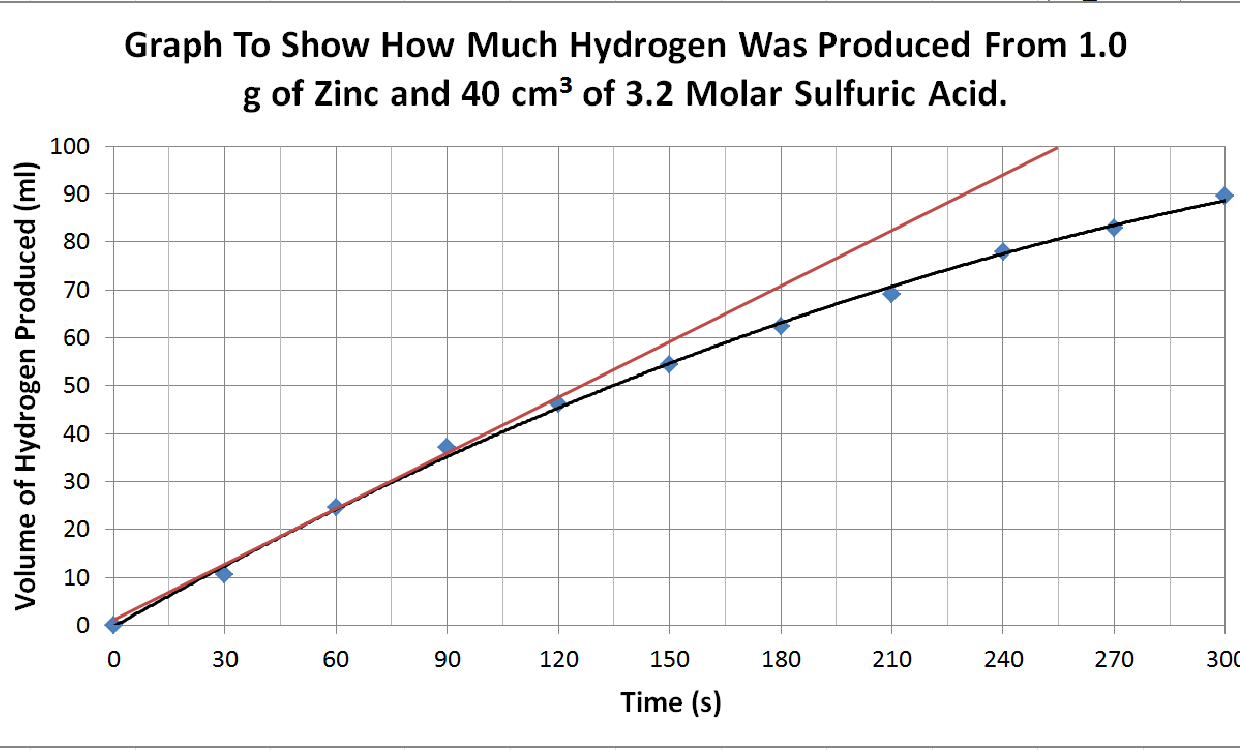
\includegraphics[width=\textwidth]{./Analysis/Images/1NonCatalyst/32Molar.pdf}
    \caption{3.2 Molar Sulfuric Acid and 1.0 g of Zinc Average Graph} \label{fig:32MolarSAGradient}
\end{figure}

$Gradient = \frac{100}{227.14}$

Therefore:

$Rate = 0.440 \; ml \; s^{-1}$

This graph appears to start curving off as time goes on, thus meaning that the reaction gets slower over time. This shape can be explained by the fact that as the reaction progresses, there are less reactants available to react and therefore as stated by collision theory, the rate of reaction will decrease. This is discussed in more detail in section \ref{factors} on page \pageref{factors}. For a reaction to occur, molecules must collide with enough kinetic energy in order to overcome the repulsive and bonding forces of the molecule. Therefore as there will be less reactants in a given amount of space, there will be less chance of molecules colliding, thus making the reaction less likely as time goes on. 

\begin{figure}[H]
    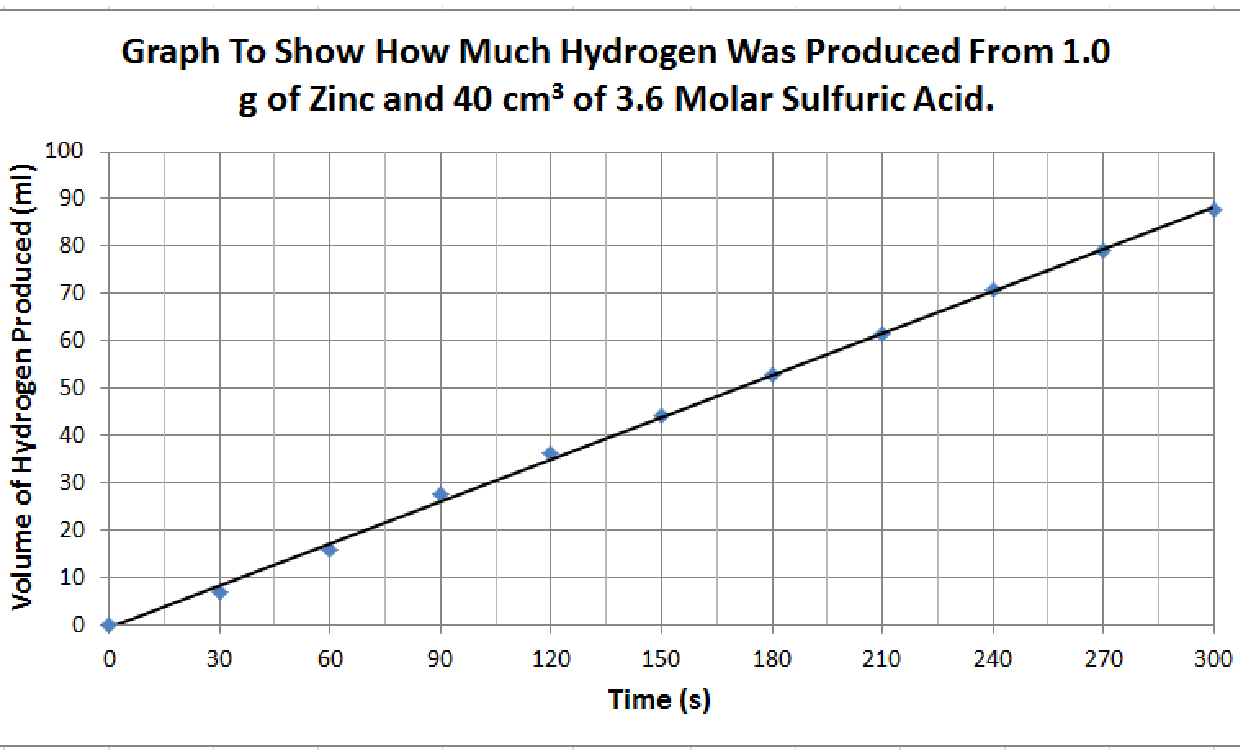
\includegraphics[width=\textwidth]{./Analysis/Images/1NonCatalyst/36Molar.pdf}
    \caption{3.6 Molar Sulfuric Acid and 1.0 g of Zinc Average Graph} \label{fig:36MolarSAGradient}
\end{figure}

$Gradient = \frac{87.67}{300}$

Therefore:

$Rate = 0.292 \; ml \; s^{-1}$

\begin{figure}[H]
    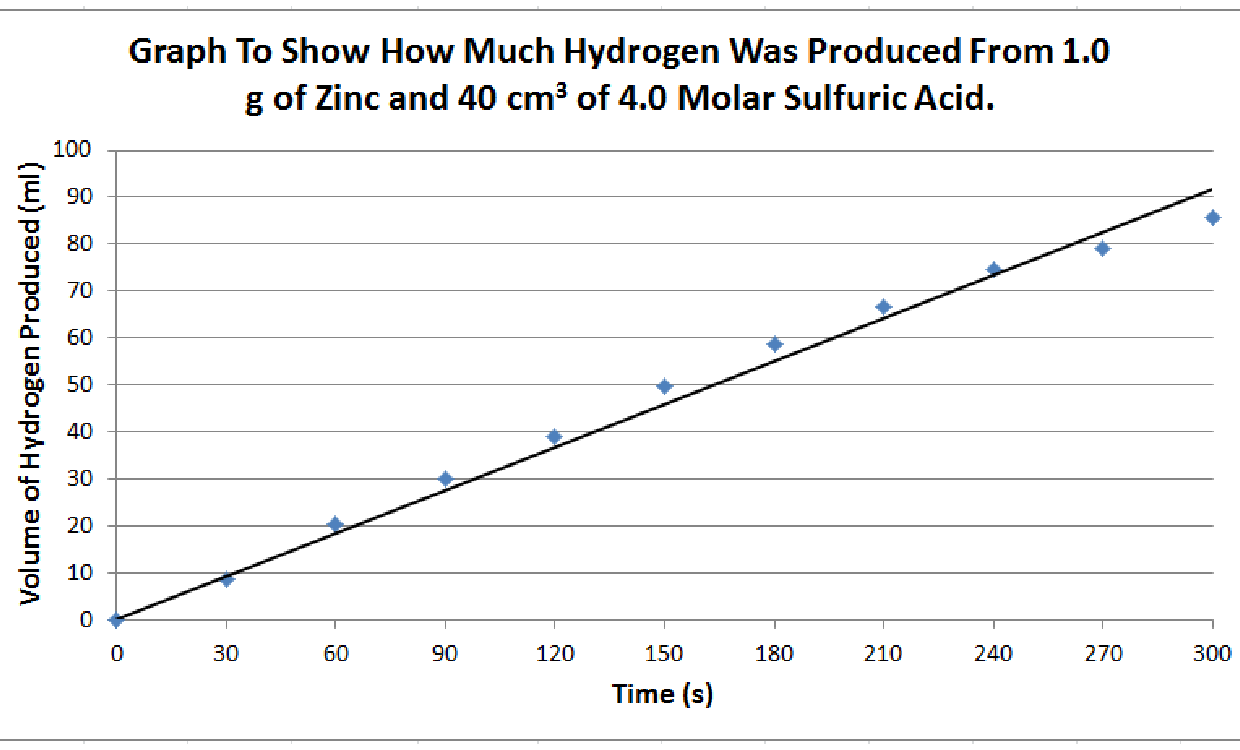
\includegraphics[width=\textwidth]{./Analysis/Images/1NonCatalyst/40Molar.pdf}
    \caption{4.0 Molar Sulfuric Acid and 1.0 g of Zinc Average Graph} \label{fig:40MolarSAGradient}
\end{figure}

$Gradient = \frac{92}{300}$

Therefore:

$Rate = 0.307 \; ml \; s^{-1}$

Below the rates of reactions are summarised in a table.

\begin{figure}[H]
    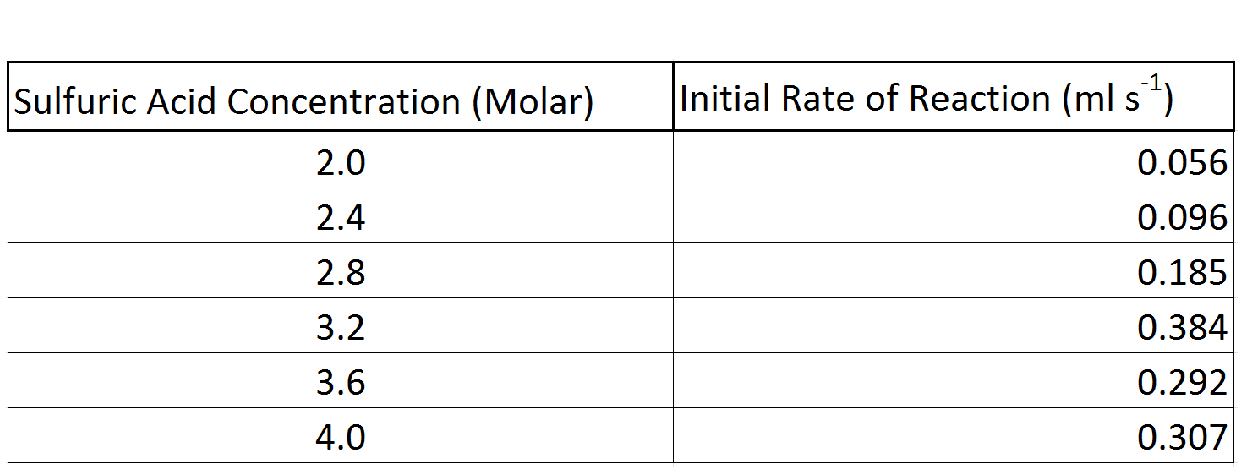
\includegraphics[width=\textwidth]{./Analysis/Images/1NonCatalyst/Rates.pdf}
    \caption{Initial Rates of Reactions for the Non-Catalysed Zinc and Sulfuric Acid Reaction} \label{fig:RatesSA}
\end{figure}

Below the rates of reactions are compiled into a rate vs concentration graph.

\begin{figure}[H]
    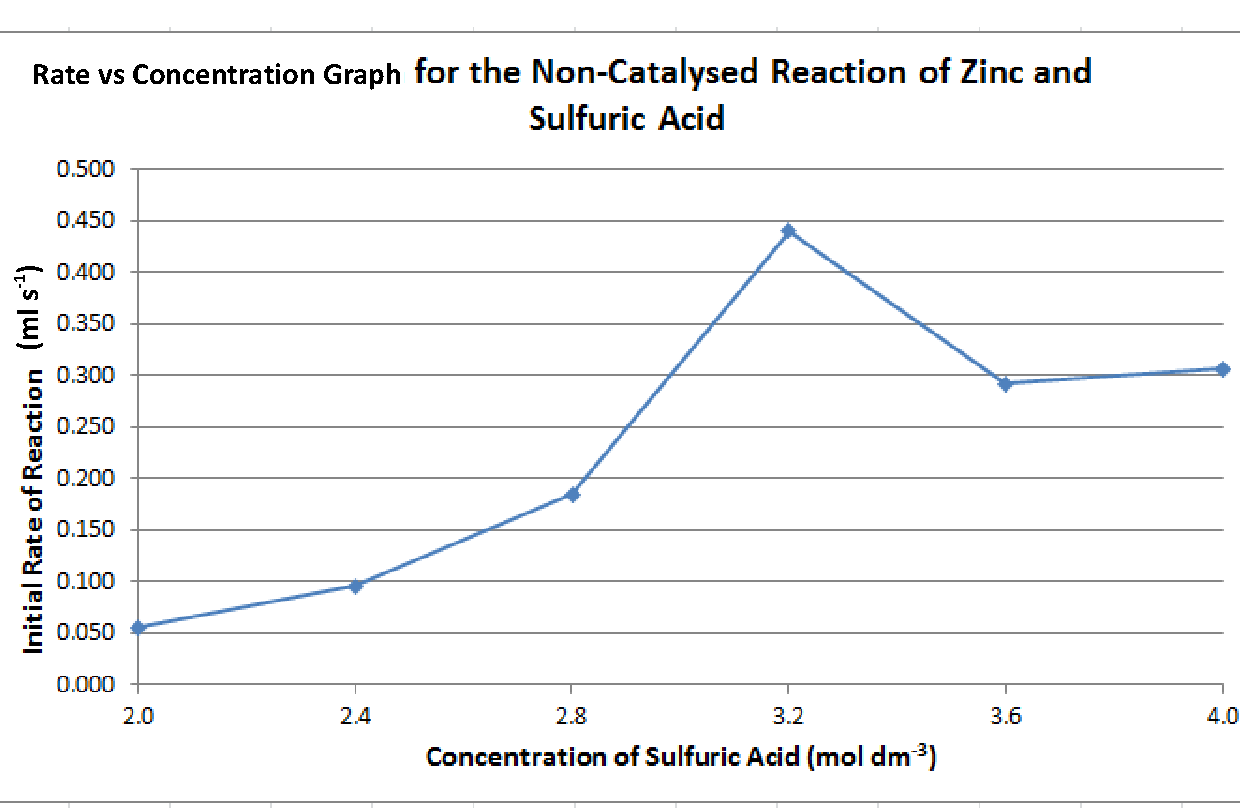
\includegraphics[width=\textwidth]{./Analysis/Images/1NonCatalyst/ProgressGraph.pdf}
    \caption{Rate vs Concentration Graph for the Non-Catalysed Reaction} \label{fig:ProgressGraphSA}
\end{figure}

The rate vs concentration graph for this experiment appears to be a second order reaction up to 3.2 Molar; however I believe that the zinc clumps at higher concentrations of acids, which would explain the decreased rate of reaction after 3.2 molar. Therefore I think that the order of sulfuric acid without the presence of a catalyst is second order. This means that doubling the concentration of sulfuric acid in this reaction quadruples the initial rate of reaction. The rate equation for this reaction would be:

$Rate = k [Sulfuric Acid]^2$

In order to work out the rate constant of this equation, the equation has to be re-arranged to:

$k = \frac{Rate}{[Sulfuric Acid]^2}$

By putting my experimental result from the 2.8 molar concentration series into the equation you get:

$k = \frac{0.185}{2.8^2}$

Therefore the rate constant 'k' is equal to 0.0236 to 3 significant figures.

I have identified a possible mechanism for the production of hydrogen from the uncatalysed reaction of zinc and sulfuric acid. This is illustrated in the following diagram.

\begin{figure}[H]
    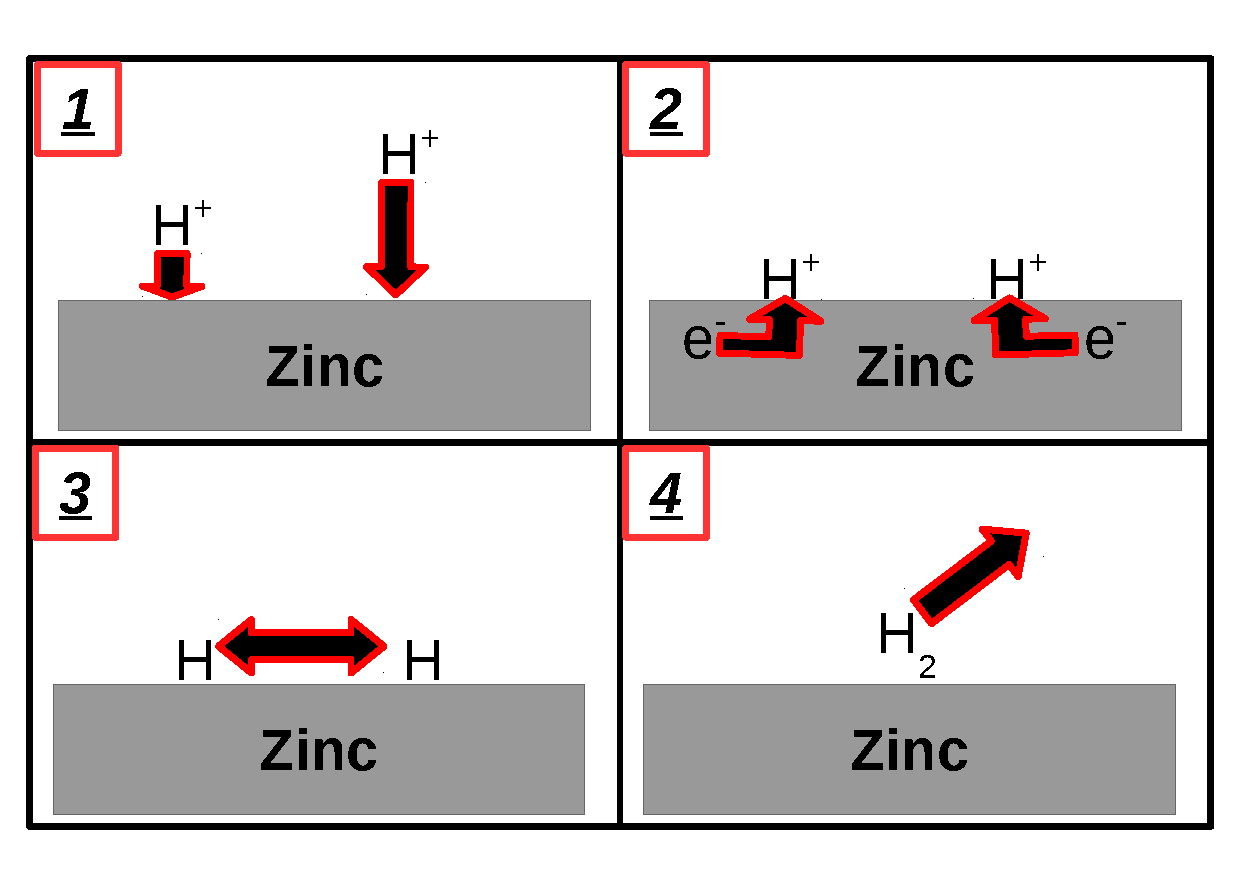
\includegraphics[width=\textwidth]{./Analysis/Images/UncatalysedMechanism.pdf}
    \caption{Proposed mechanism for the zinc acid reaction} \label{fig:uncatalysedMechanism}
\end{figure}

\begin{enumerate}
\item Hydrogen ions supplied from the acid arrive at the powdered zinc's surface area.
\item Electrons supplied from the zinc reduce hydrogen the hydrogen ions on the zincs surface area, thus oxidising the zinc.
\item Hydrogen atoms form a covalent bond with each other to form a molecule of hydrogen gas.
\item The hydrogen gas moves away from the zincs surface area.
\end{enumerate}

From the proposed mechanism, the rate determining step can be





%FINISH MECHANISM!














\section{Zinc and Sulfuric Acid With a Copper Sulfate Catalyst} 


	\subsection{Sulfuric Acid}

Below are the graphs that I have used to work out the rate of the reaction for the experiment series that did involve a catalyst but varied in sulfuric acid concentration. All graphs have taken a mean average of the three repeats in order to plot the data points. As discussed in my 'Chosen Method' section on page \pageref{Chosen Method} I am using the equation $Gradient = \frac{Change in Y}{Change in X}$ and as the gradient is equal to the rate of reaction, I will be able to use the graphs below in order to generate a rate vs concentration graph which will determine the order of the reaction. I will calculate all rates to 3 decimal places.


\begin{figure}[H]
    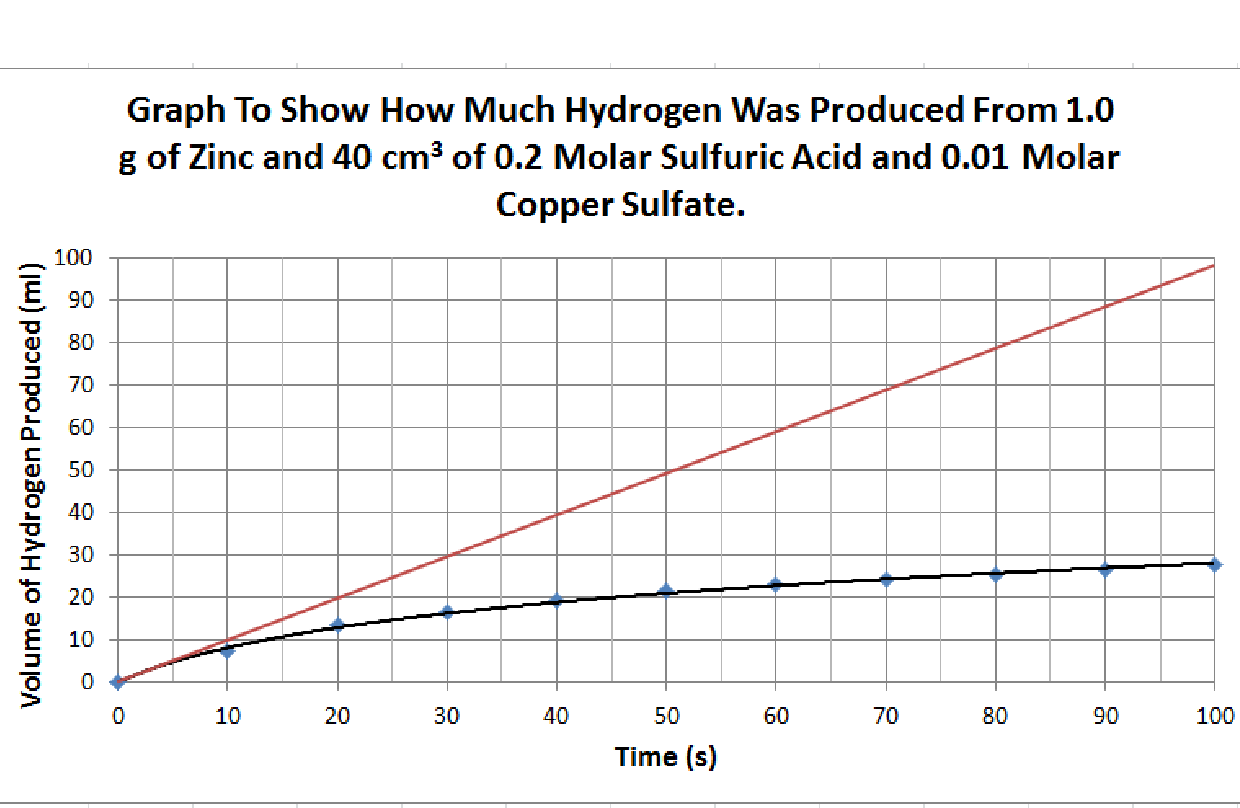
\includegraphics[width=\textwidth]{./Analysis/Images/2Catalysed/02Molar.pdf}
    \caption{0.2 Molar Sulfuric Acid and 0.01 Molar Copper Sulfate and 1.0 g of Zinc Average Graph} \label{fig:02MolarSACSGradient}
\end{figure}

$Gradient = \frac{97}{100}$

Therefore:

$Rate = 0.970 \; ml \; s^{-1}$

\begin{figure}[H]
    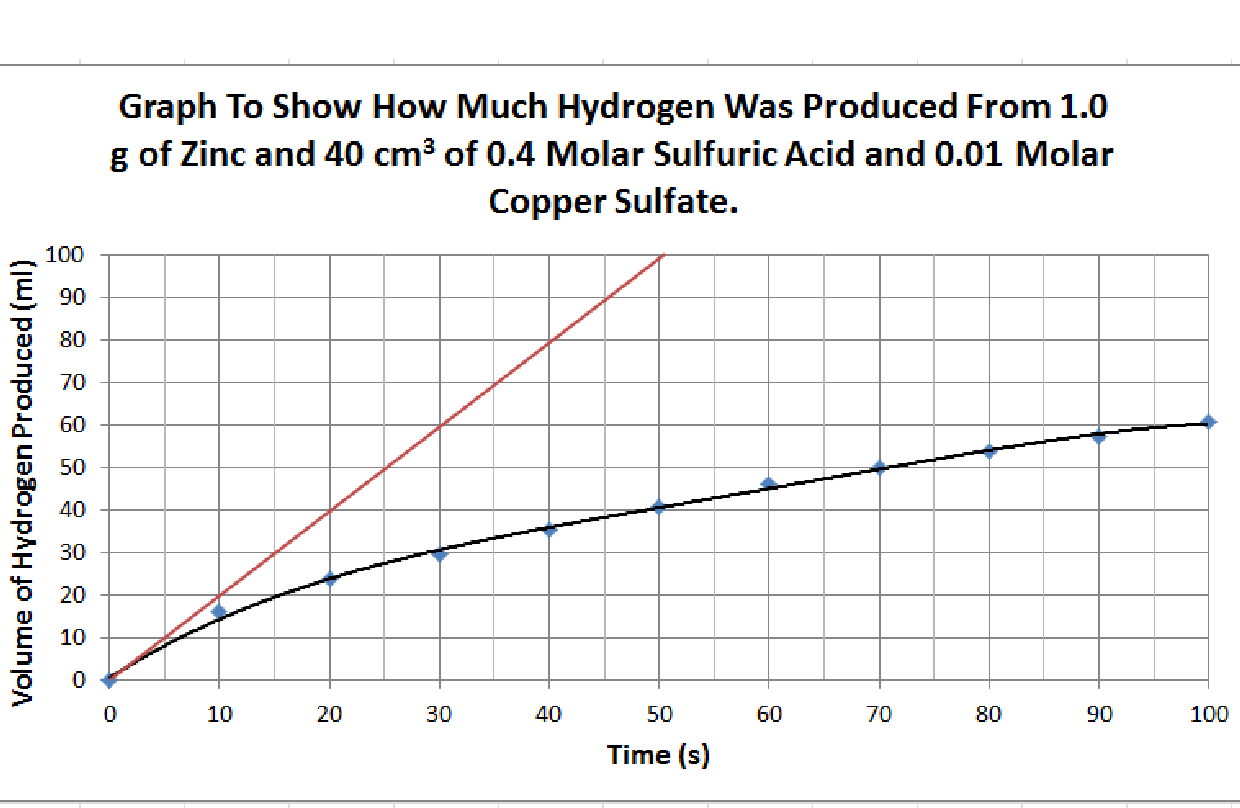
\includegraphics[width=\textwidth]{./Analysis/Images/2Catalysed/04Molar.pdf}
    \caption{0.4 Molar Sulfuric Acid and 0.01 Molar Copper Sulfate and 1.0 g of Zinc Average Graph} \label{fig:04MolarSACSGradient}
\end{figure}

$Gradient = \frac{100}{51.5}$

Therefore:

$Rate = 1.942 \; ml \; s^{-1}$

\begin{figure}[H]
    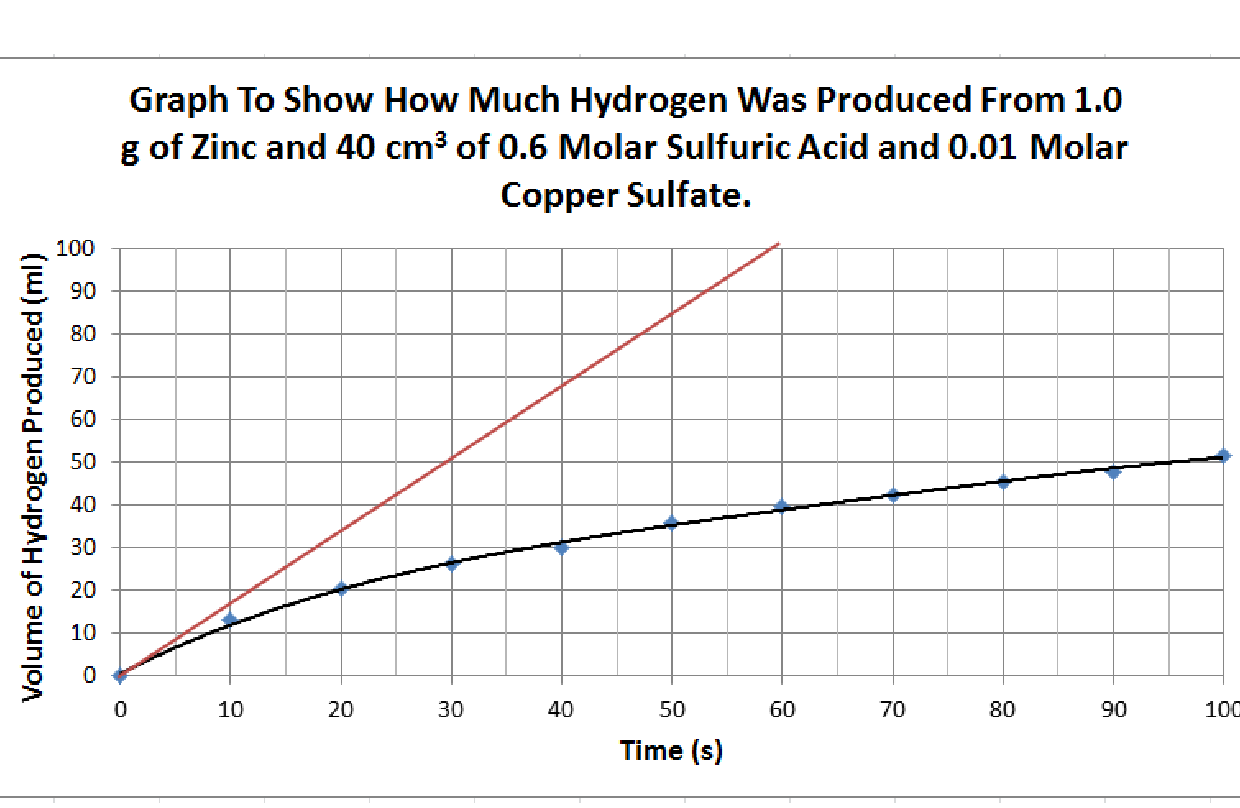
\includegraphics[width=\textwidth]{./Analysis/Images/2Catalysed/06Molar.pdf}
    \caption{0.6 Molar Sulfuric Acid and 0.01 Molar Copper Sulfate and 1.0 g of Zinc Average Graph} \label{fig:06MolarSACSGradient}
\end{figure}

$Gradient = \frac{100}{59}$

Therefore:

$Rate = 1.695 \; ml \; s^{-1}$

\begin{figure}[H]
    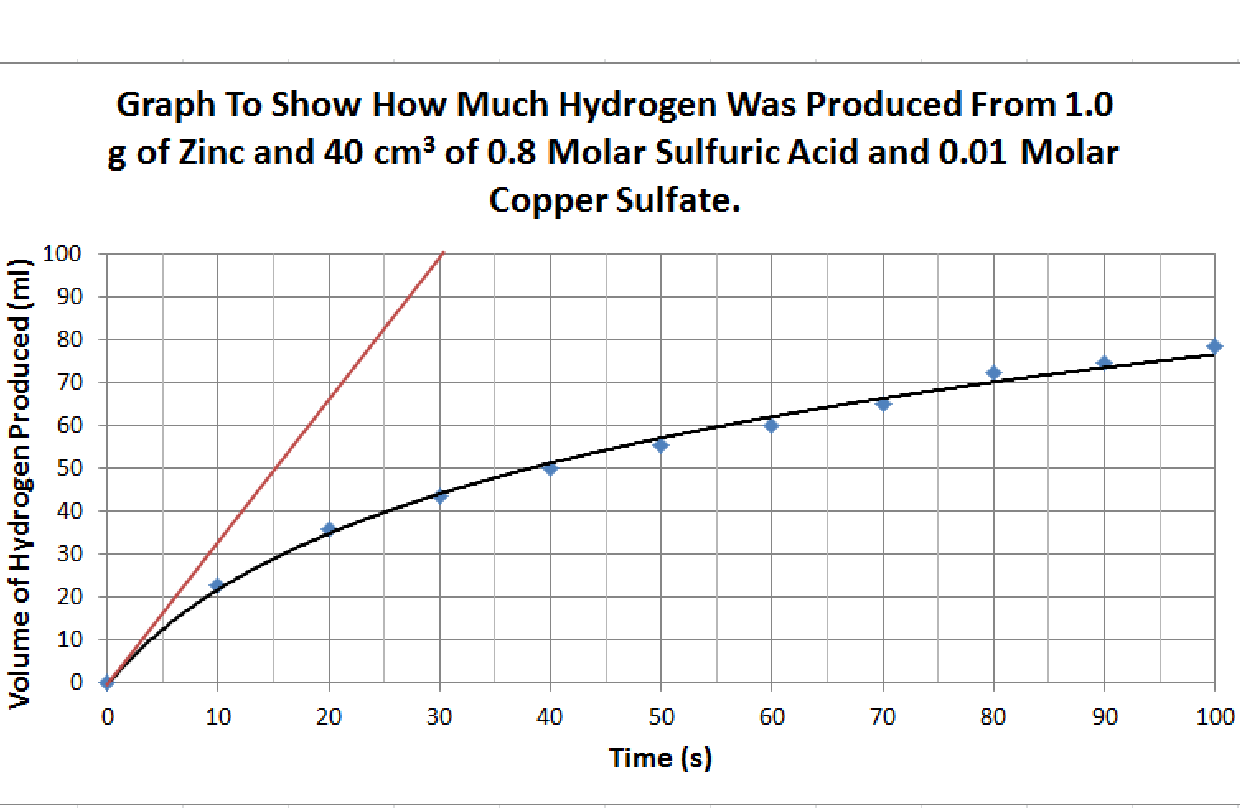
\includegraphics[width=\textwidth]{./Analysis/Images/2Catalysed/08Molar.pdf}
    \caption{0.8 Molar Sulfuric Acid and 0.01 Molar Copper Sulfate and 1.0 g of Zinc Average Graph} \label{fig:08MolarSACSGradient}
\end{figure}

$Gradient = \frac{100}{30.7}$

Therefore:

$Rate = 3.257 \; ml \; s^{-1}$

\begin{figure}[H]
    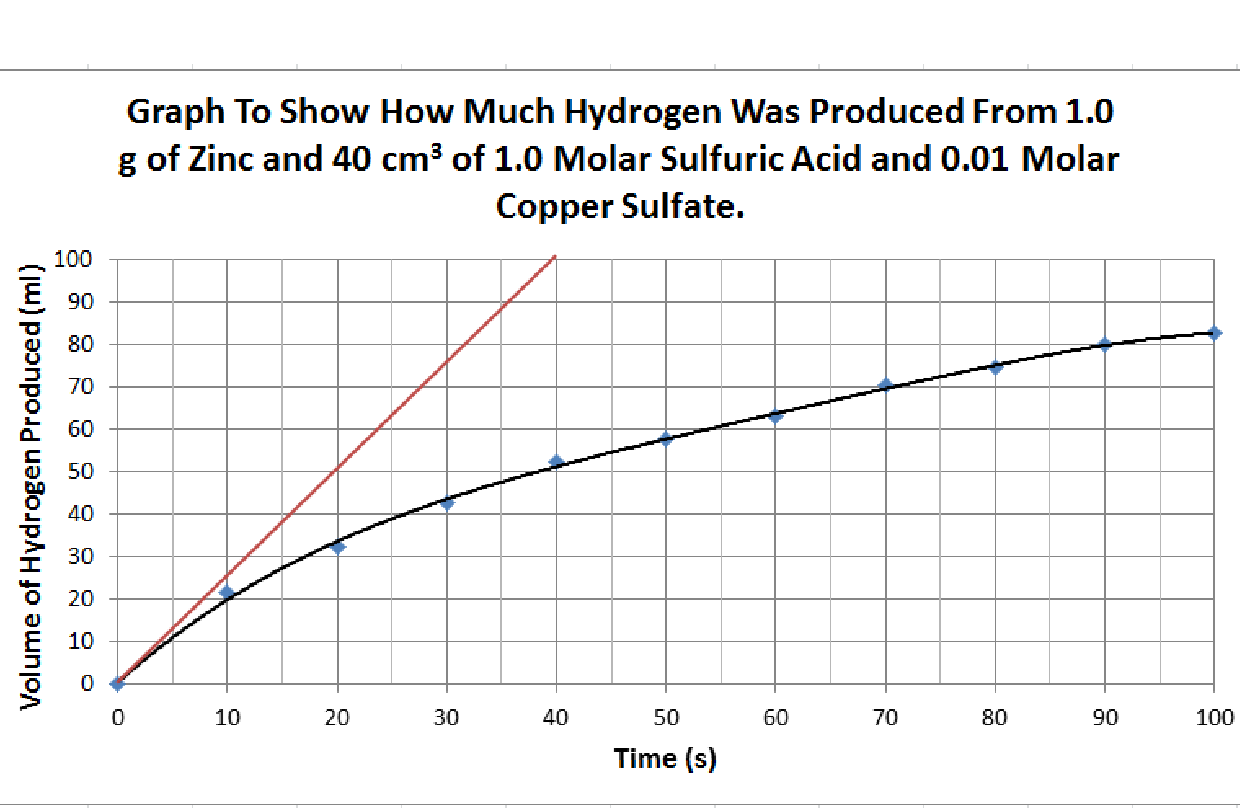
\includegraphics[width=\textwidth]{./Analysis/Images/2Catalysed/10Molar.pdf}
    \caption{1.0 Molar Sulfuric Acid and 0.01 Molar Copper Sulfate and 1.0 g of Zinc Average Graph} \label{fig:10MolarSACSGradient}
\end{figure}

$Gradient = \frac{100}{40}$

Therefore:

$Rate = 2.500 \; ml \; s^{-1}$

\begin{figure}[H]
    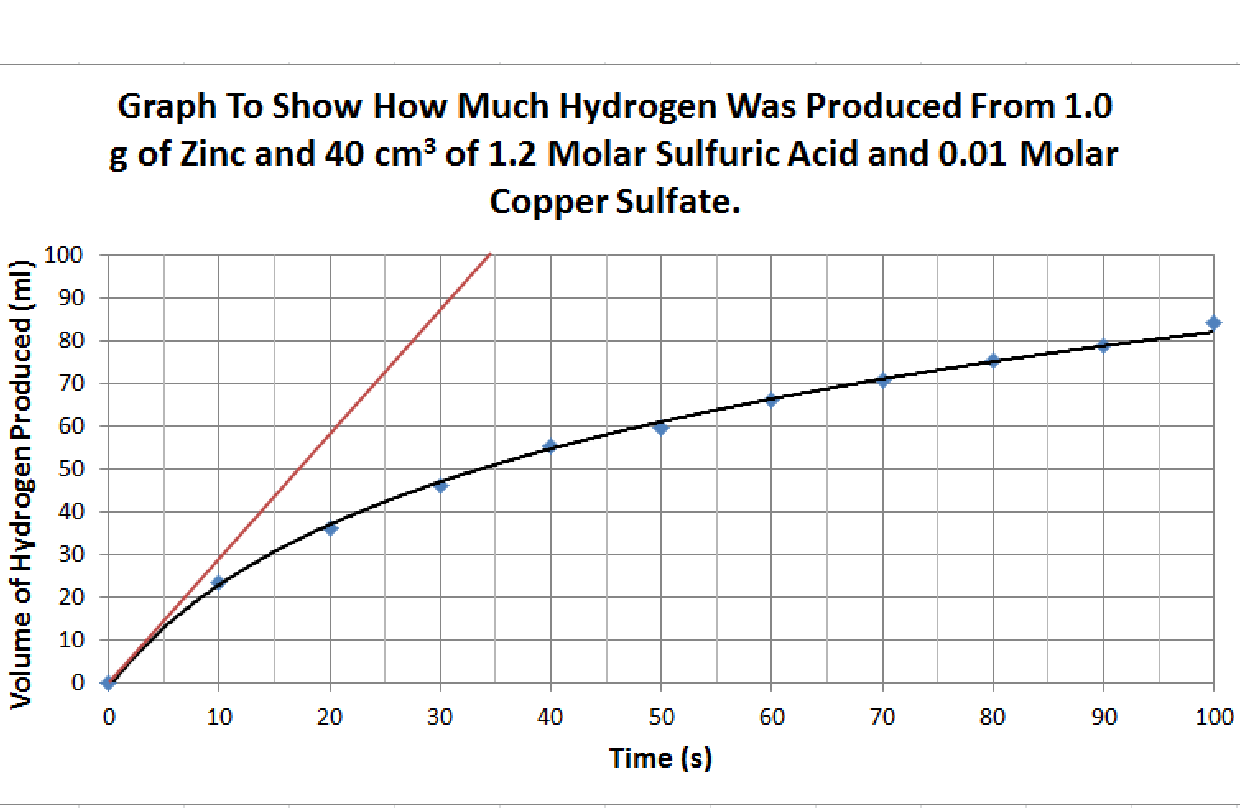
\includegraphics[width=\textwidth]{./Analysis/Images/2Catalysed/12Molar.pdf}
    \caption{1.2 Molar Sulfuric Acid and 0.01 Molar Copper Sulfate and 1.0 g of Zinc Average Graph} \label{fig:12MolarSACSGradient}
\end{figure}

$Gradient = \frac{100}{34.5}$

Therefore:

$Rate = 2.899 \; ml \; s^{-1}$

Below the rates of reactions are summarised in a table.

\begin{figure}[H]
    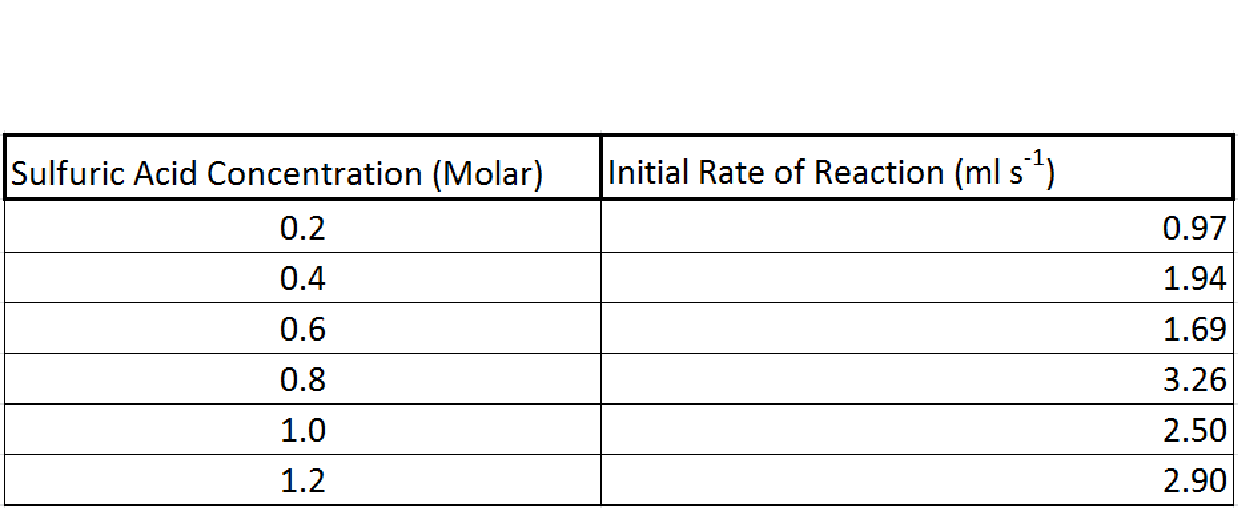
\includegraphics[width=\textwidth]{./Analysis/Images/2Catalysed/Rates.pdf}
    \caption{Initial Rates of Reactions for the Catalysed Zinc and Sulfuric Acid Reaction} \label{fig:RatesSACS}
\end{figure}

Below the rates of reactions are compiled into a rate vs concentration graph.

\begin{figure}[H]
    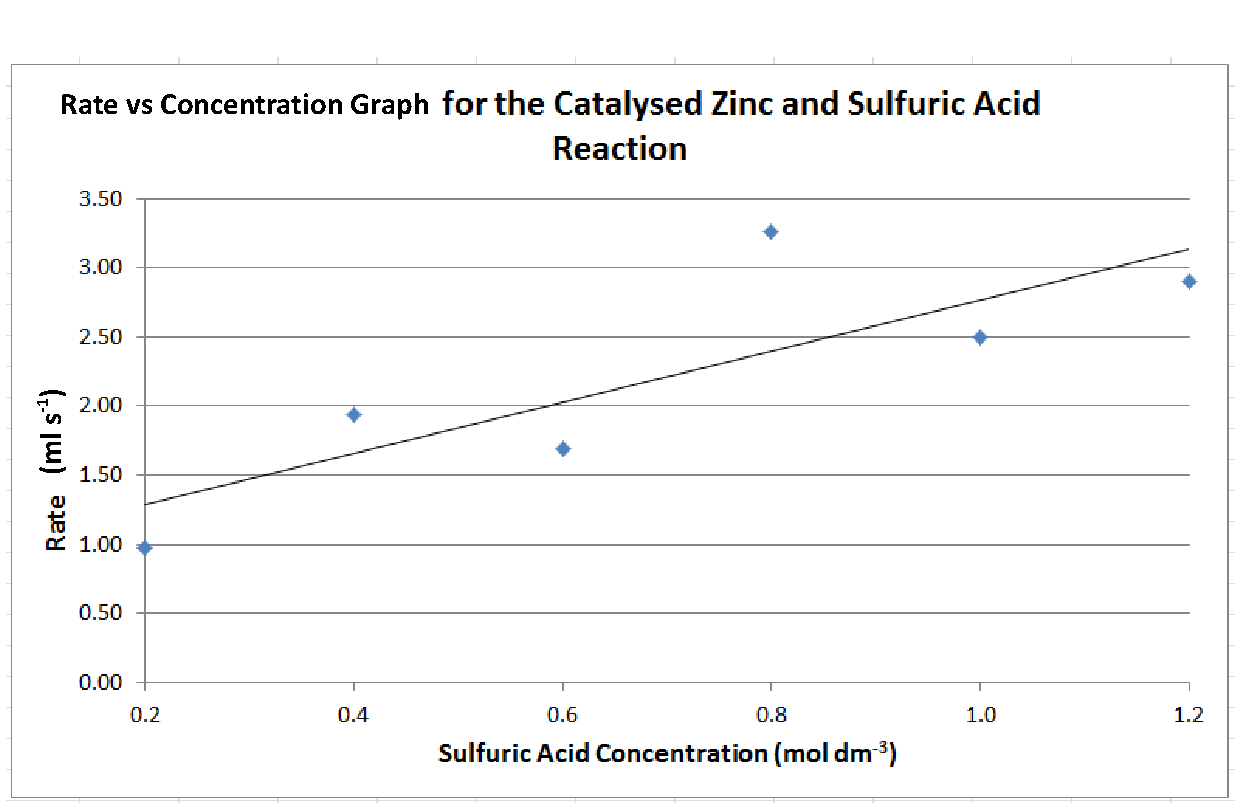
\includegraphics[width=\textwidth]{./Analysis/Images/2Catalysed/ProgressGraph.pdf}
    \caption{Rate vs Concentration Graph for the Catalysed Zinc and Sulfuric Acid Reaction} \label{fig:ProgressGraphSACS}
\end{figure}

The rate vs concentration graph for this experiment is too scattered to get an accurate result; however due to the scattered result it appears that a straight line of best fit would be most appropriate. Therefore I believe that the when in the presence of copper sulfate, sulfuric acid is a first order reactant.This means that doubling the concentration of sulfuric acid in this reaction doubles the initial rate of reaction. The rate equation for this reaction would be:

$Rate = k [Sulfuric Acid]$

Next I will work out if copper sulfate is also part of the rate equation.

	\subsection{Copper Sulfate}
Below are the graphs that I have used to work out the rate of the reaction for the experiment series that did involve a catalyst and varied in copper sulfate concentration. All graphs have taken a mean average of the three repeats in order to plot the data points. As discussed in my 'Chosen Method' section on page \pageref{Chosen Method} I am using the equation $Gradient = \frac{Change in Y}{Change in X}$ and as the gradient is equal to the rate of reaction, I will be able to use the graphs below in order to generate a rate vs concentration graph which will determine the order of the reaction. I will calculate all rates to 3 decimal places.


\begin{figure}[H]
    \includegraphics[width=\textwidth]{./Analysis/Images/3VaryCopperSulfate/001Molar.pdf}
    \caption{0.4 Molar Sulfuric Acid and 0.01 Molar Copper Sulfate and 1.0 g of Zinc Average Graph} \label{fig:001VaryCopperSulfate}
\end{figure}

$Gradient = \frac{70}{58}$

Therefore:

$Rate = 1.207 \; ml \; s^{-1}$

\begin{figure}[H]
    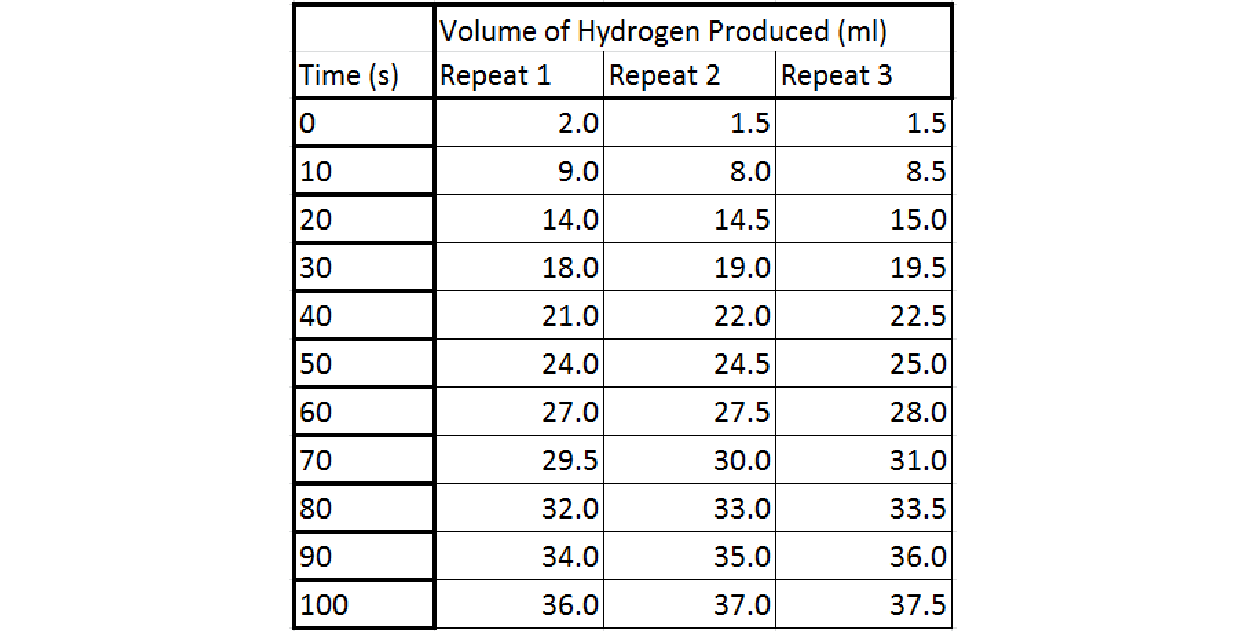
\includegraphics[width=\textwidth]{./Analysis/Images/3VaryCopperSulfate/002Molar.pdf}
    \caption{0.4 Molar Sulfuric Acid and 0.02 Molar Copper Sulfate and 1.0 g of Zinc Average Graph} \label{fig:002VaryCopperSulfate}
\end{figure}

$Gradient = \frac{79}{90}$

Therefore:

$Rate = 0.778 \; ml \; s^{-1}$

\begin{figure}[H]
    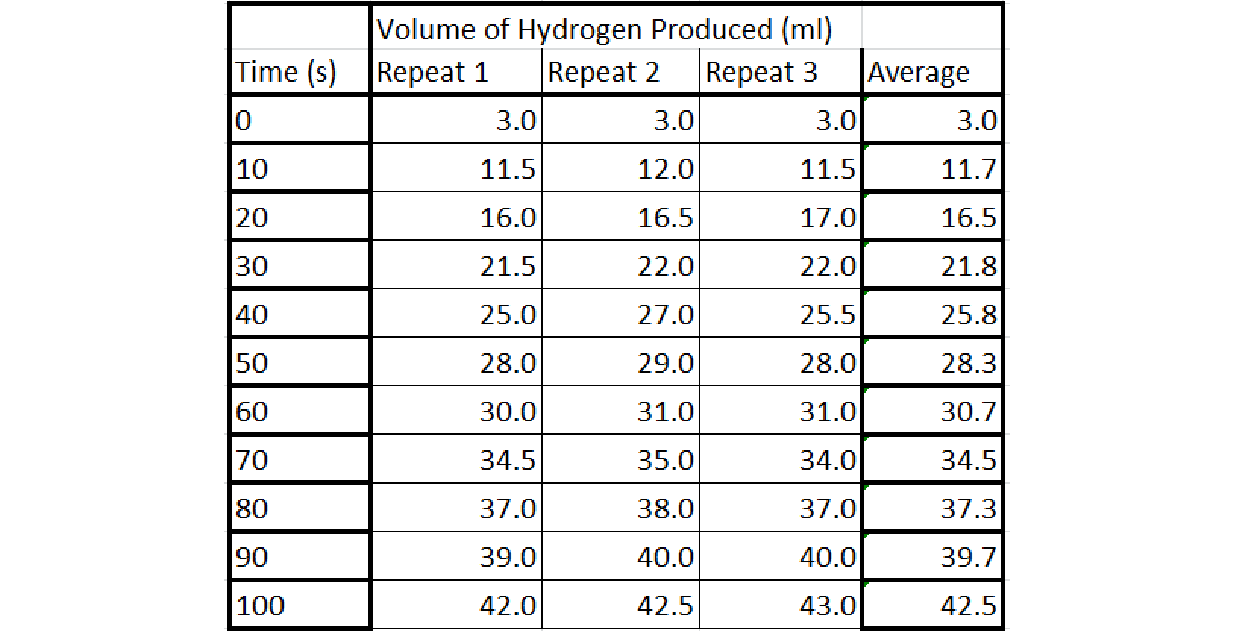
\includegraphics[width=\textwidth]{./Analysis/Images/3VaryCopperSulfate/003Molar.pdf}
    \caption{0.4 Molar Sulfuric Acid and 0.03 Molar Copper Sulfate and 1.0 g of Zinc Average Graph} \label{fig:003VaryCopperSulfate}
\end{figure}

$Gradient = \frac{70}{60}$

Therefore:

$Rate = 1.167 \; ml \; s^{-1}$

\begin{figure}[H]
    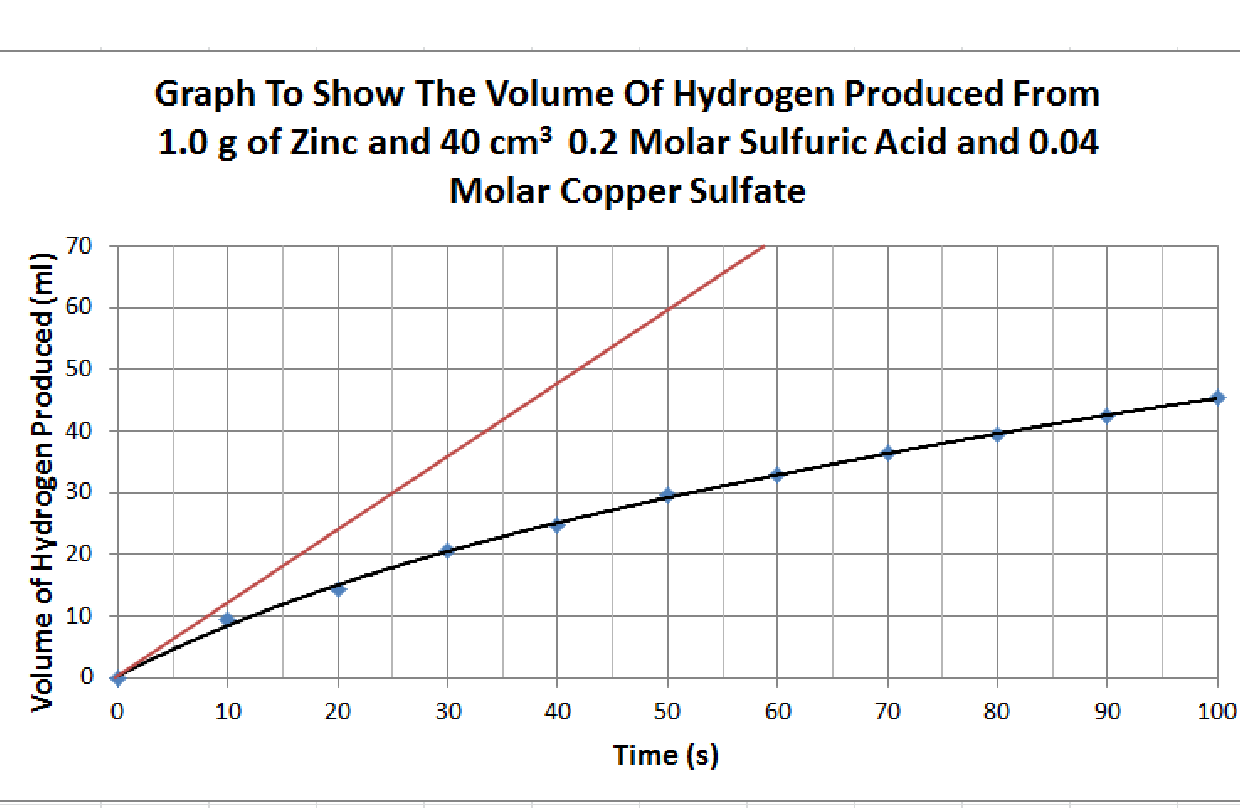
\includegraphics[width=\textwidth]{./Analysis/Images/3VaryCopperSulfate/004Molar.pdf}
    \caption{0.4 Molar Sulfuric Acid and 0.04 Molar Copper Sulfate and 1.0 g of Zinc Average Graph} \label{fig:004VaryCopperSulfate}
\end{figure}

$Gradient = \frac{70}{57.5}$

Therefore:

$Rate = 1.217 \; ml \; s^{-1}$

\begin{figure}[H]
    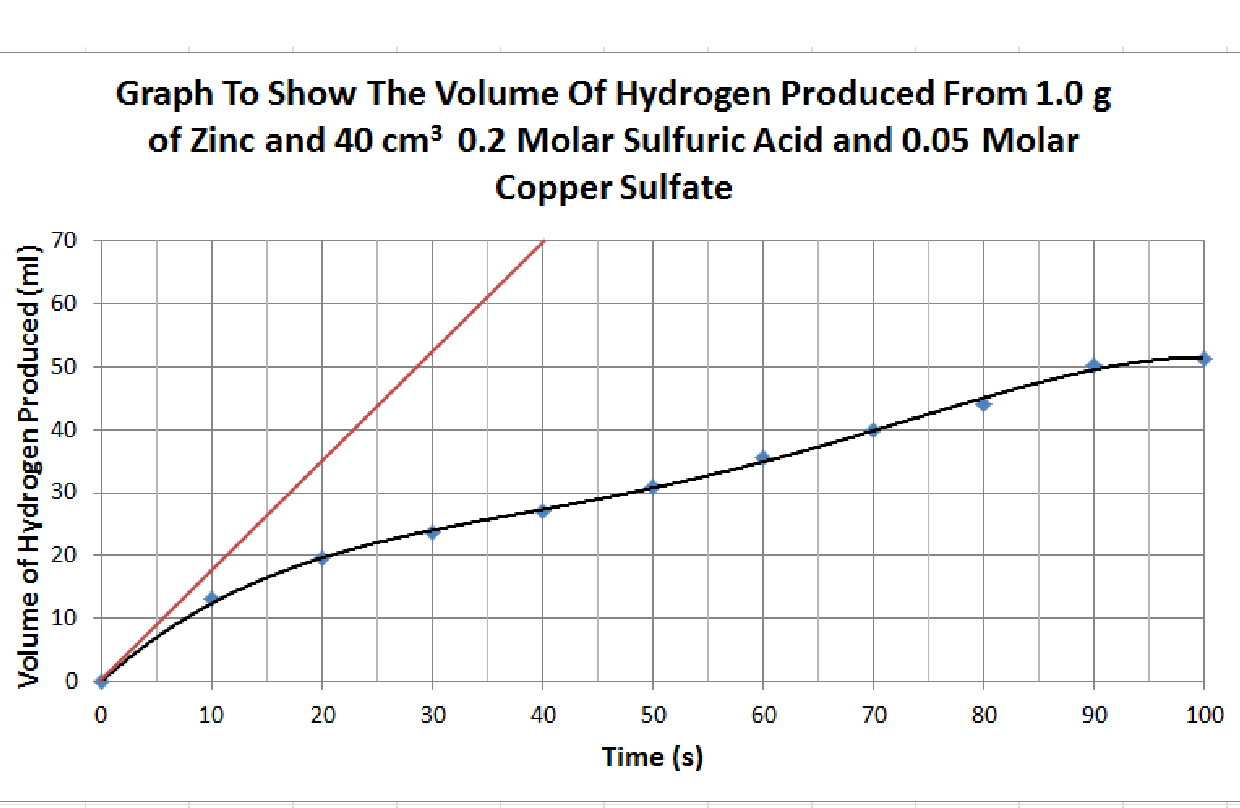
\includegraphics[width=\textwidth]{./Analysis/Images/3VaryCopperSulfate/005Molar.pdf}
    \caption{0.4 Molar Sulfuric Acid and 0.05 Molar Copper Sulfate and 1.0 g of Zinc Average Graph} \label{fig:005VaryCopperSulfate}
\end{figure}

$Gradient = \frac{70}{40}$

Therefore:

$Rate = 1.750 \; ml \; s^{-1}$

\begin{figure}[H]
    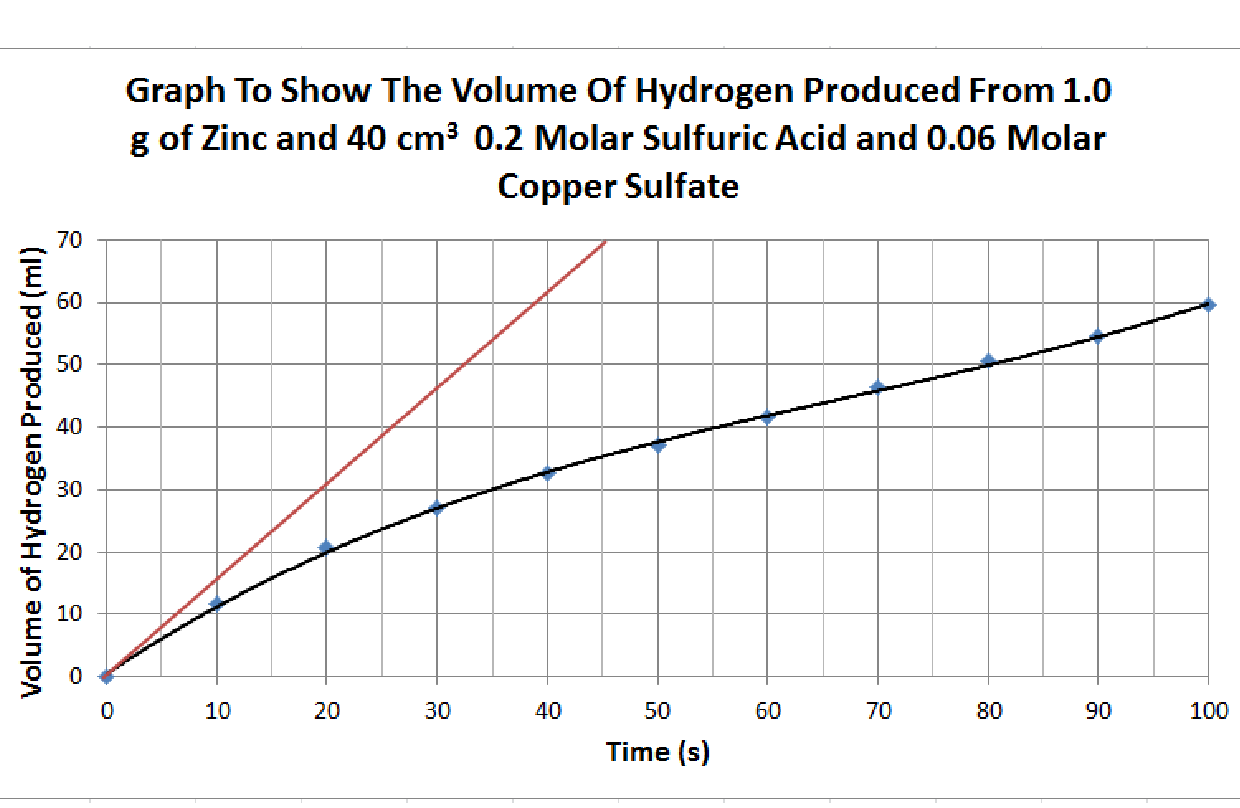
\includegraphics[width=\textwidth]{./Analysis/Images/3VaryCopperSulfate/006Molar.pdf}
    \caption{0.4 Molar Sulfuric Acid and 0.06 Molar Copper Sulfate and 1.0 g of Zinc Average Graph} \label{fig:006VaryCopperSulfate}
\end{figure}
$Gradient = \frac{70}{45}$

Therefore:

$Rate = 1.556 \; ml \; s^{-1}$

Below the rates of reactions are summarised in a table.

\begin{figure}[H]
    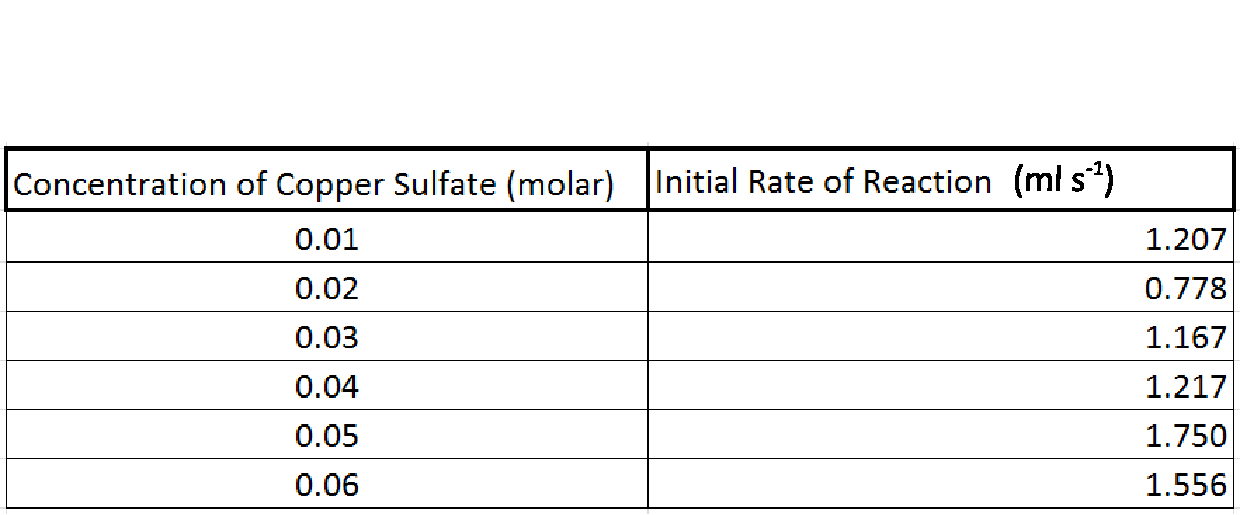
\includegraphics[width=\textwidth]{./Analysis/Images/3VaryCopperSulfate/Rates.pdf}
    \caption{Initial Rates of Reactions for the Catalysed Zinc and Sulfuric Acid Reaction} \label{fig:RatesSACSVary}
\end{figure}

Below the rates of reactions are compiled into a rate vs concentration graph.

\begin{figure}[H]
    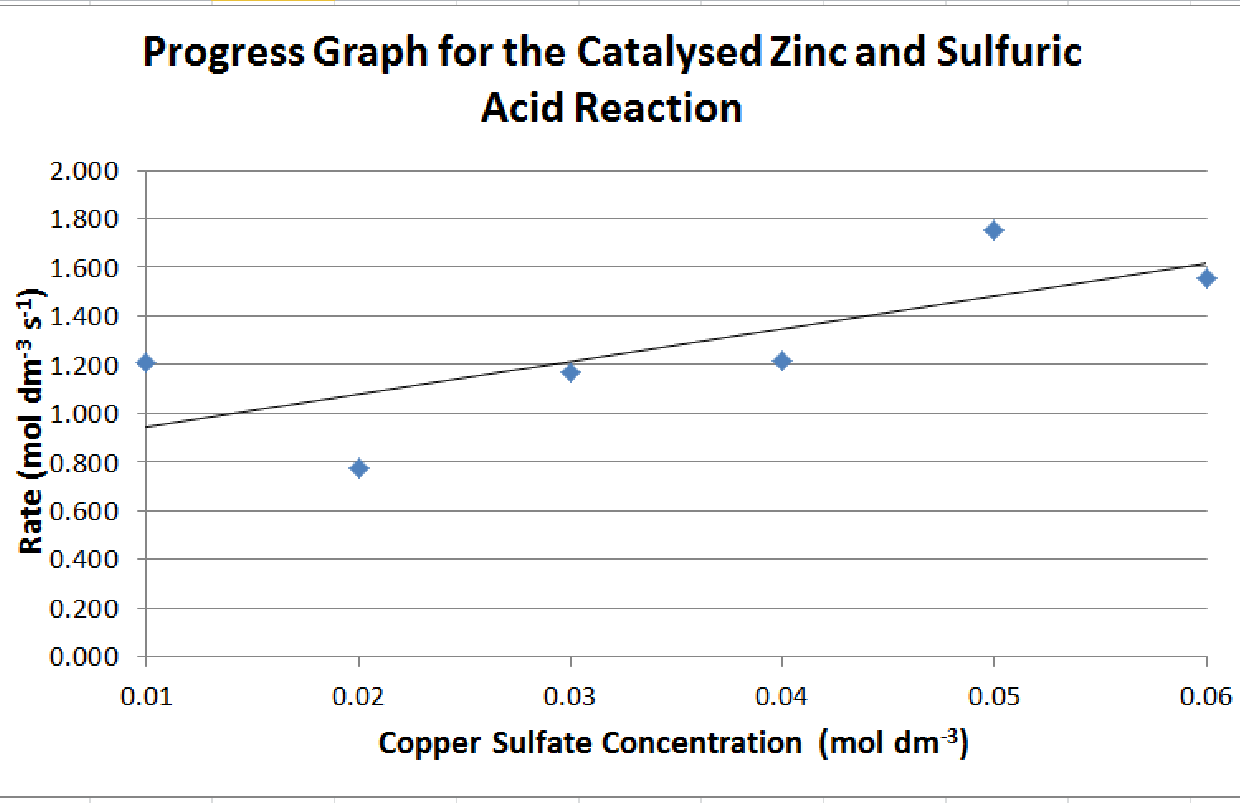
\includegraphics[width=\textwidth]{./Analysis/Images/3VaryCopperSulfate/ProgressGraph.pdf}
    \caption{Rate vs Concentration Graph for the Catalysed Zinc and Sulfuric Acid Reaction} \label{fig:ProgressGraphSACSVary}
\end{figure}

The rate vs concentration graph for this experiment, again,  is too scattered to get an accurate result; however due to the scattered result it appears that a straight line of best fit would be most appropriate. Therefore I believe that the copper sulfate is a first order reactant. This means that doubling the concentration of copper sulfate in this reaction doubles the initial rate of reaction. The rate equation for this overall reaction would be:

$Rate = k [Sulfuric Acid] [Copper Sulfate]$

This means that overall the reaction is a second order reaction and both individual reactants are first order reactants.






%MECHANISM








\section{Comparing Catalysts}

The copper sulfate graph can be found on page \pageref{fig:04MolarSACSGradient}, Figure \ref{fig:04MolarSACSGradient}.

\begin{figure}[H]
    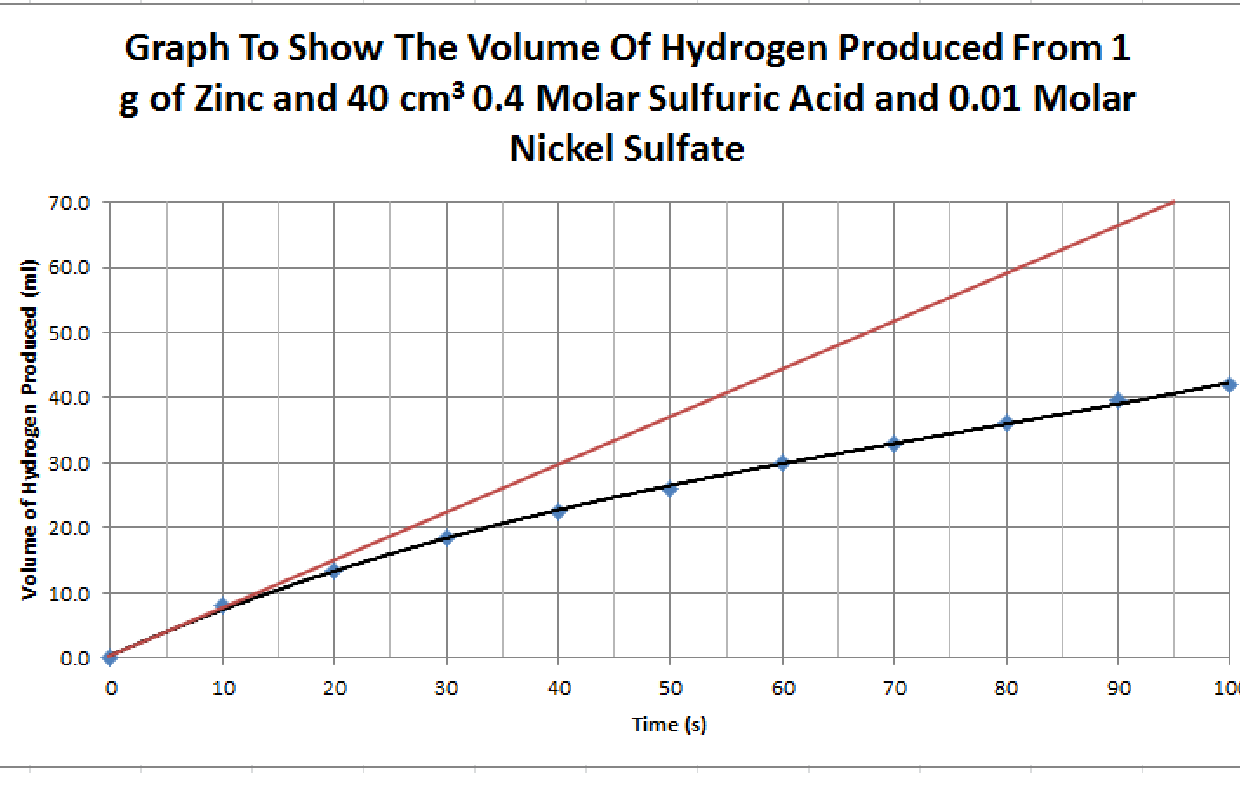
\includegraphics[width=\textwidth]{./Analysis/Images/4DifferentCatalysts/Nickel.pdf}
    \caption{0.4 Molar Sulfuric Acid and 0.01 Molar Nickel Sulfate and 1.0 g of Zinc Average Graph} \label{fig:NickelGradient}
\end{figure}

\begin{figure}[H]
    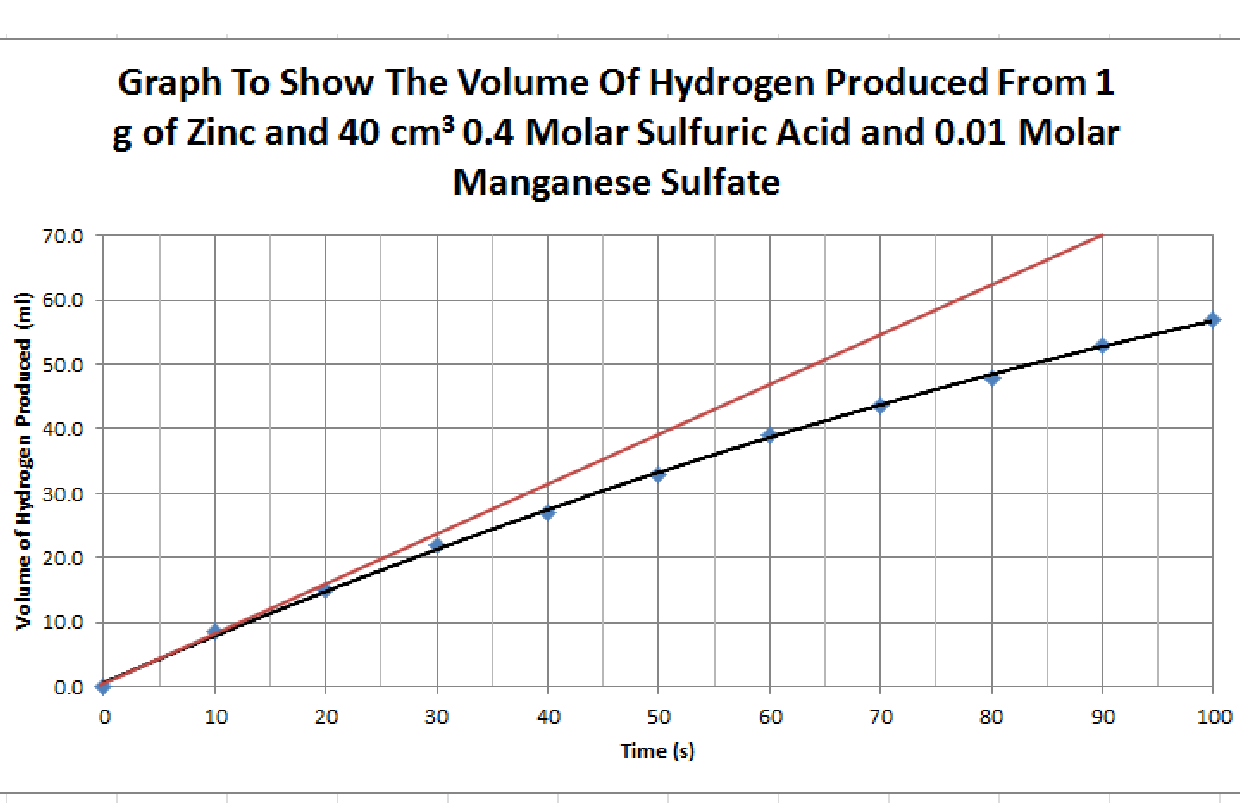
\includegraphics[width=\textwidth]{./Analysis/Images/4DifferentCatalysts/Manganese.pdf}
    \caption{0.4 Molar Sulfuric Acid and 0.01 Molar Manganese Sulfate and 1.0 g of Zinc Average Graph} \label{fig:ManganeseGradient}
\end{figure}

\begin{figure}[H]
    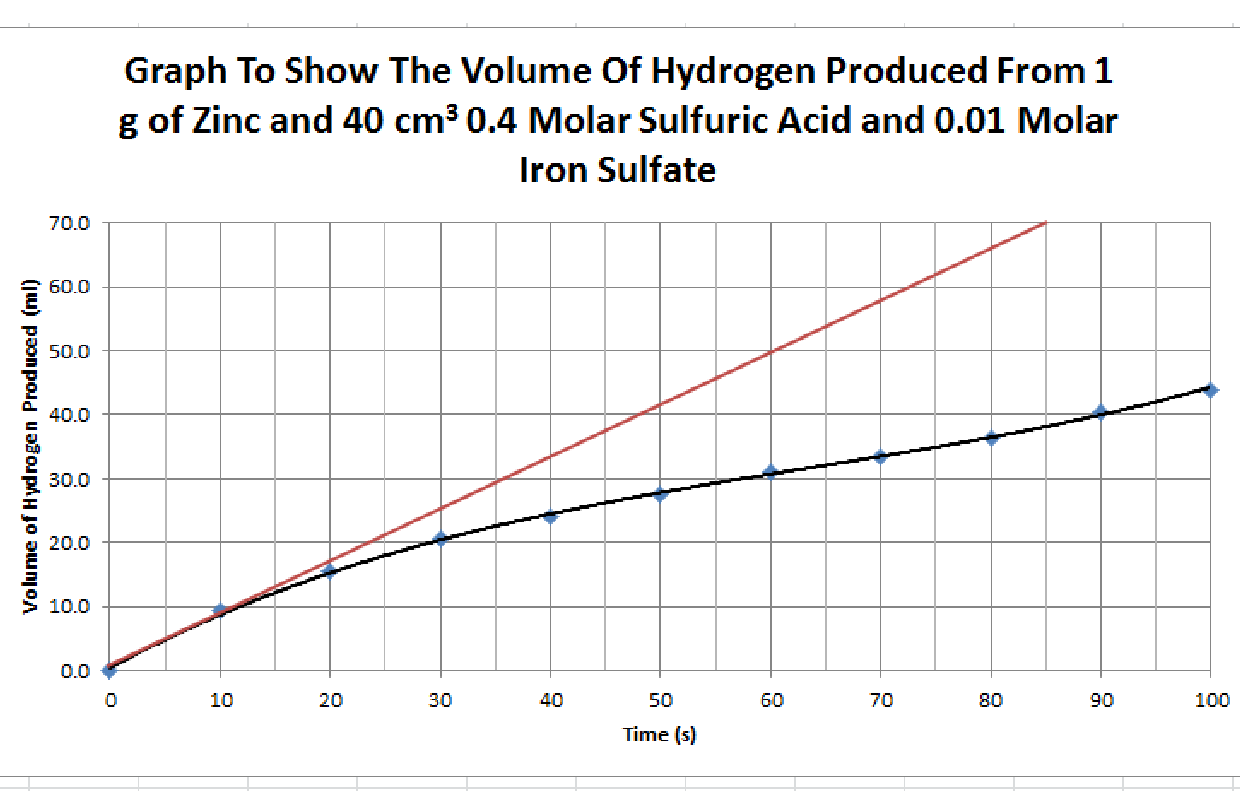
\includegraphics[width=\textwidth]{./Analysis/Images/4DifferentCatalysts/Iron.pdf}
    \caption{0.4 Molar Sulfuric Acid and 0.01 Molar Iron Sulfate and 1.0 g of Zinc Average Graph} \label{fig:IronGradient}
\end{figure}

Below the rates of reactions are summarised in a table.

\begin{figure}[H]
    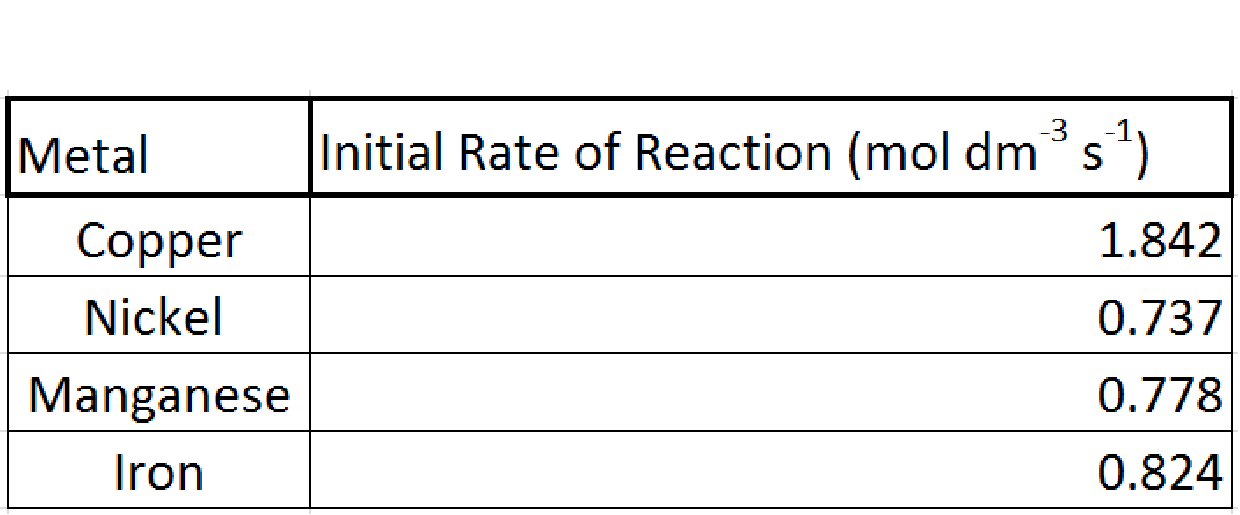
\includegraphics[width=\textwidth]{./Analysis/Images/4DifferentCatalysts/Rates.pdf}
    \caption{Initial Rates of Reactions for the Different Catalysts Tested} \label{fig:RatesDiffCat}
\end{figure}


 For this experiment I have created a bar chart to compare the rate of reaction, this can be seen below.

\begin{figure}[H]
    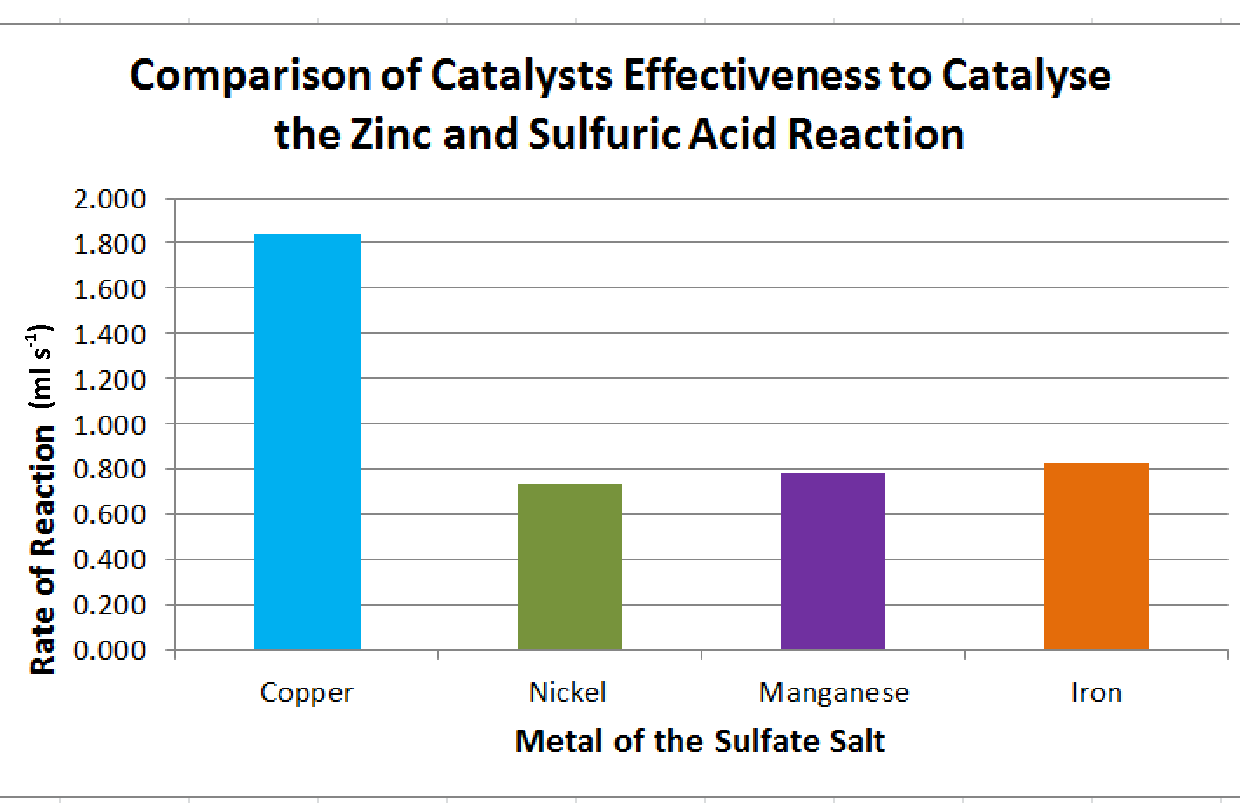
\includegraphics[width=\textwidth]{./Analysis/Images/4DifferentCatalysts/Comparison.pdf}
    \caption{Comparison of Rates of Different Sulfate Catalysts} \label{fig:ComparisonCat}
\end{figure}

This experiment has shown that copper sulfate is the most effective catalyst, which has over double the rate of all the other sulfates. Iron is the next most effective catalyst followed by manganese and then nickel.

I believe that copper is the most effective catalyst as the electrolytic cell that it creates works so well together as the copper is not as reactive as zinc. 

Catalysts which are of similar reactivity to zinc (iron and nickel) do not create an as efficient electrolytic cell as that of copper which is significantly less reactive than zinc. By having the catalyst significantly less reactive than zinc the electrolytic cell becomes more efficient at producing hydrogen as hydrogen ions are going to be reduced to form hydrogen gas (one of the products of a metal and acid reaction) at the less reactive electrode. This leads to an increased production of hydrogen gas. The manganese sulfate result can be explained by the fact that manganese is more reactive than zinc, and therefore does not cause an increase in production of hydrogen in the same way as the other catalysts tested. I think that this is the reason that copper sulfate is a significantly more efficient catalyst.

\section{Investigating the Solubility of Hydrogen} 

The graph below shows all of the data points taken from the raw data table in the Experiment section of my coursework. 

\begin{figure}[H]
    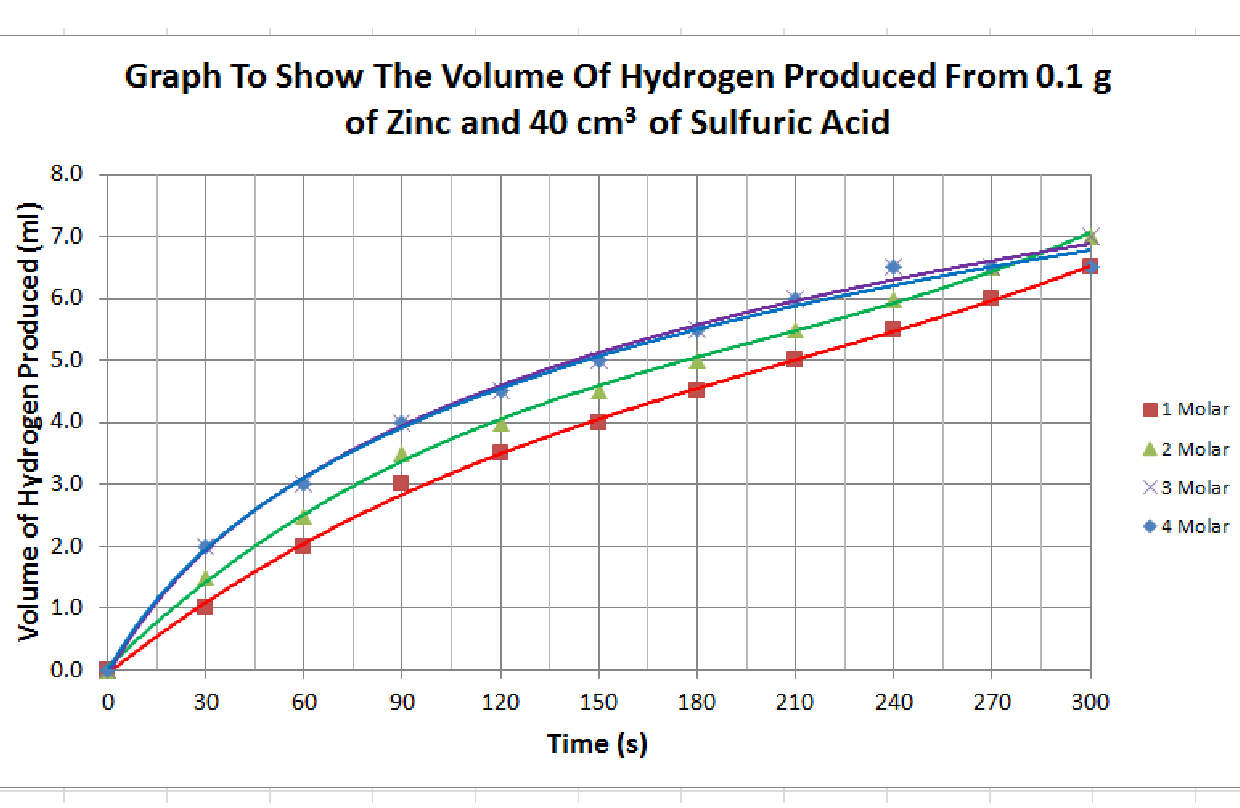
\includegraphics[width=\textwidth]{./Analysis/Images/Solubility.pdf}
    \caption{Comparison of the Hydrogen Produced When Different Concentrations of Sulfuric Acid is in Excess} \label{fig:ComparisonCat}
\end{figure}

Although there have been no scientific sources that I can find which discuss the solubility of hydrogen in higher concentrations of acids, my data starts to suggest that it does increase. At 4 molar sulfuric acid the volume of hydrogen produced is less than that of the lower concentrations which suggests that solubility of hydrogen does increase. Therefore the higher the concentration of the acid, the less accurate the results are as some of the hydrogen is dissolving into the solution. But to confidently comment on this, I would have to carry out the experiment with a wider range of acid concentrations and repeats. 

From the equation of the reaction (Zn (s) + H$_2$SO$_4$ (aq) $\rightarrow$ ZnSO$_4$ (aq) + H$_2$ (g)) you can work out that that by using 40 cm$^3$ of 4 molar sulfuric acid, the zinc is over 100x greater in excess. This calculation is shown below.

Moles of sulfuric acid:
\begin{itemize}
\item $Number \; of \; Moles = Concentration \times Volume$
\item $0.16 = 4 \times (40 \times 10^{-3})$
\end{itemize}

Moles of zinc:
\begin{itemize}
\item $Number \; of \; Moles = \frac{Mass}{Molecular Mass}$
\item $0.001529285 = \frac{0.1}{65.39}$
\end{itemize}

Therefore there are over 100 more sulfuric acid particles than zinc. The total volume of hydrogen that can be produced by the reaction is 36.70 cm$^3$. This can be worked out as the stoichiometry between zinc and hydrogen is a ratio of 1:1 and therefore the number of moles of hydrogen that can be produced is equal to the number of moles of the zinc (as the acid is in excess). This leaves the equation to be:

Volume of hydrogen produced:
\begin{itemize}
\item $Volume = Number \; of \;  Moles \times 24$
\item $0.03670284 \; dm^3 = 0.001529285 \times 24$
\item $36.70284 \; cm^3$
\end{itemize}

Obviously my results has produced less hydrogen than expected for a number of reasons. First of all I only measured the volume of hydrogen produced over 5 minutes. Secondly, some hydrogen will have been produced before the bung was placed into the conical flask. Finally the zincs surface area to volume ratio isn't are large as it could be, therefore not producing as much hydrogen as possible.

